\begin{event}{CIRM Conference: Free Computational Mathematics}{CIRM}{CIRM, Luminy, France, 11--15 Feb 2019}{UB,UK,UG,UV,SA}{58}{17}{https://opendreamkit.org/2019/02/11/FreeComputationalMathematicsConference}

\textbf{Main goals.} \emph{Free Computational Mathematics} was
a community building and training conference for a wide mathematical audience:
it was one of the main dissemination events for \ODK and our public closing event.

\textbf{ODK implication.} This conference was organized jointly by
OpenDreamKit's sites \site{PS} and \site{UG}, under the lead of \site{PS}.
The cost was about 60\,000\,\euro, covered by \site{UK}.

\textbf{Event summary.}
We brought together users and developers of most \ODK software components
(\GAP, \Jupyter, \Linbox, \MPIR, \PariGP, \Sage, \Singular).
The workshop followed a long trend of highly productive workshops that we organised in the past,
consisting of keynote talks and hands-on tutorials with a focus on experimental research
and computational and development best practices.
There was plenty of time for interactions and collaborative work.
Part of the schedule was intentionally made up during the workshop itself,
taking input from the participants on what trainings they wanted to see.

%\textbf{Demographics.} Do you have demographic information? If so, please share!

\textbf{Results and impact.} On the dissemination side, many
participants wished for the training to extend for more than five
days, and for similar events to be organized at their location. In
particular our three participants from Nigeria went on to organize a
similar event at the University of Ibadan, with support and trainers
from OpenDreamKit (See Sage Days 102 below). On the community building
side, this was the first time that such a wide mix of developers from
PARI, Singular, GAP, LMFDB, SageMath, Oscar, and Jupyter were gathered
together and closely collaborating, which was invaluable for long term
community building.

\begin{figure}[ht]
  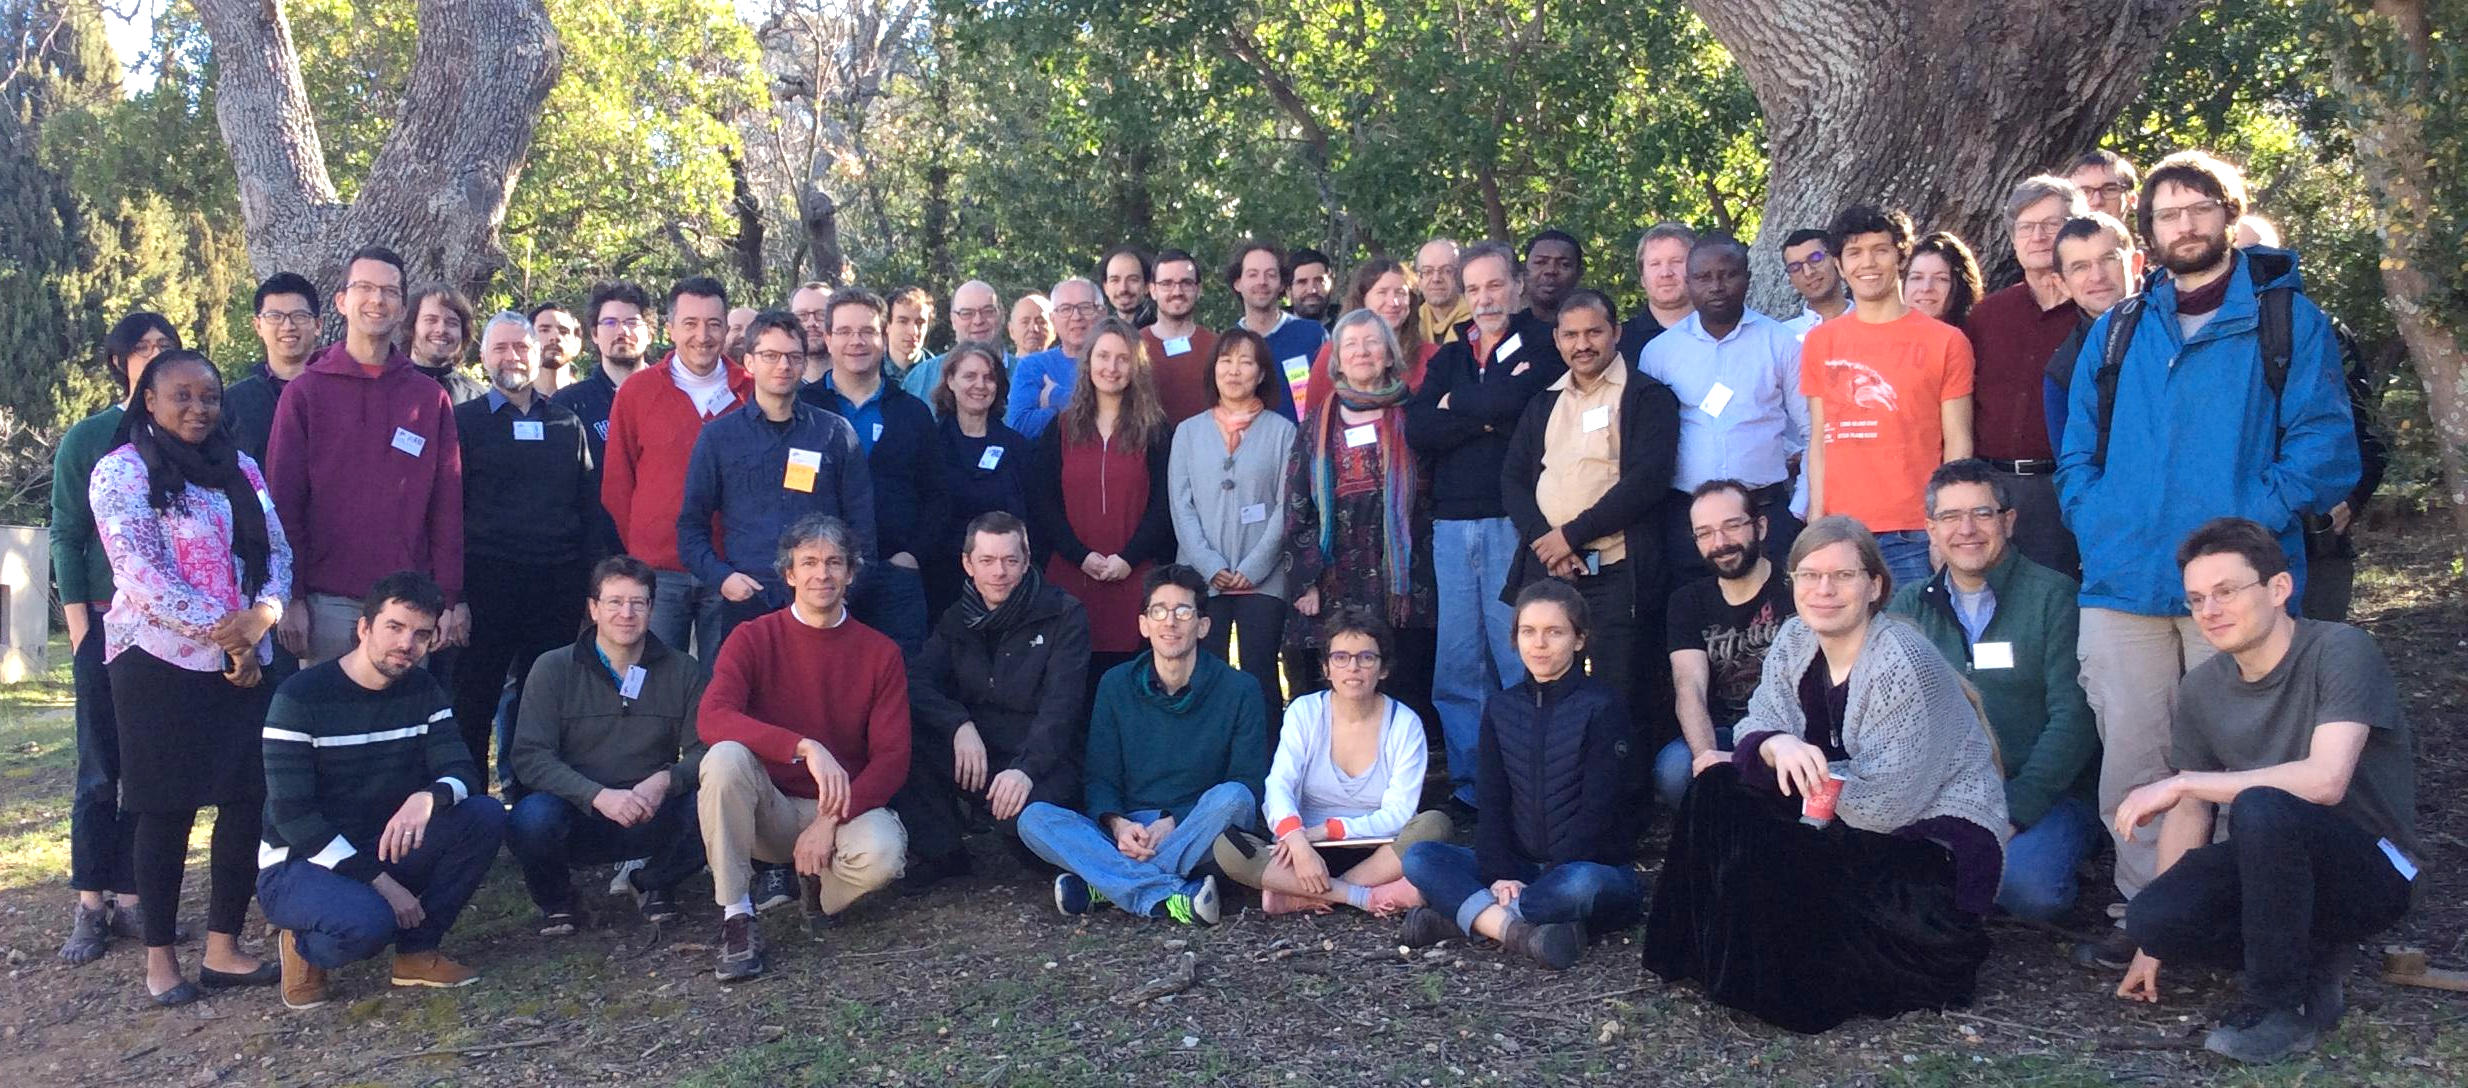
\includegraphics[width=.75\textwidth]{CIRM.jpg}
  \caption*{Free Computational Mathematics, CIRM, Luminy, France}
\end{figure}

\end{event}
